\chapter{Alternative Studies, 2018 Analysis}
\label{chap:alt_studies_2018}
This section fits different subsets of the data and compares it to the full result in 2018, similar to what was done for the 2017 analysis in \autoref{sec:data_alt_studies}. Since the model only marginally changed and the new parameters are entirely compatible with last year, we here focus on compatibility between FGD1 and FGD2, and FHC and RHC runs rather than variations in the systematics.

\section{Neutrino vs Anti-Neutrino}
In the 2017 analysis we found BeRPA to be marginally different between FHC and RHC runs, with the full data settling near the FHC result. With 1.99x more collected POT in FHC and 1.63x in RHC mode, it's interesting to see if the data subsets prefer different BeRPA models. RHC events still only make up 20\% of the total data (24795/121432), so a larger relative effect of the prior is expected.

\autoref{fig:data_fhcvsrhc_2018_fhc} shows the FHC flux parameters after the fit. We see good compatibility at low energies throughout, and the two FGDs disagreeing around 1 GeV for the \numu and \nue fluxes, returning to agreeing at 1.5 GeV. Interestingly, the FHC+RHC fit favours a higher flux normalisation at low energies than either of the separate fits (115\% vs 109\%), but still sit within the parameter error. The difference at 1 GeV manifests by the FHC+RHC fit sitting between the two, slightly towards the FHC data fit.
\begin{figure}[h]
	\centering
	\begin{subfigure}[t]{0.10\textwidth}
		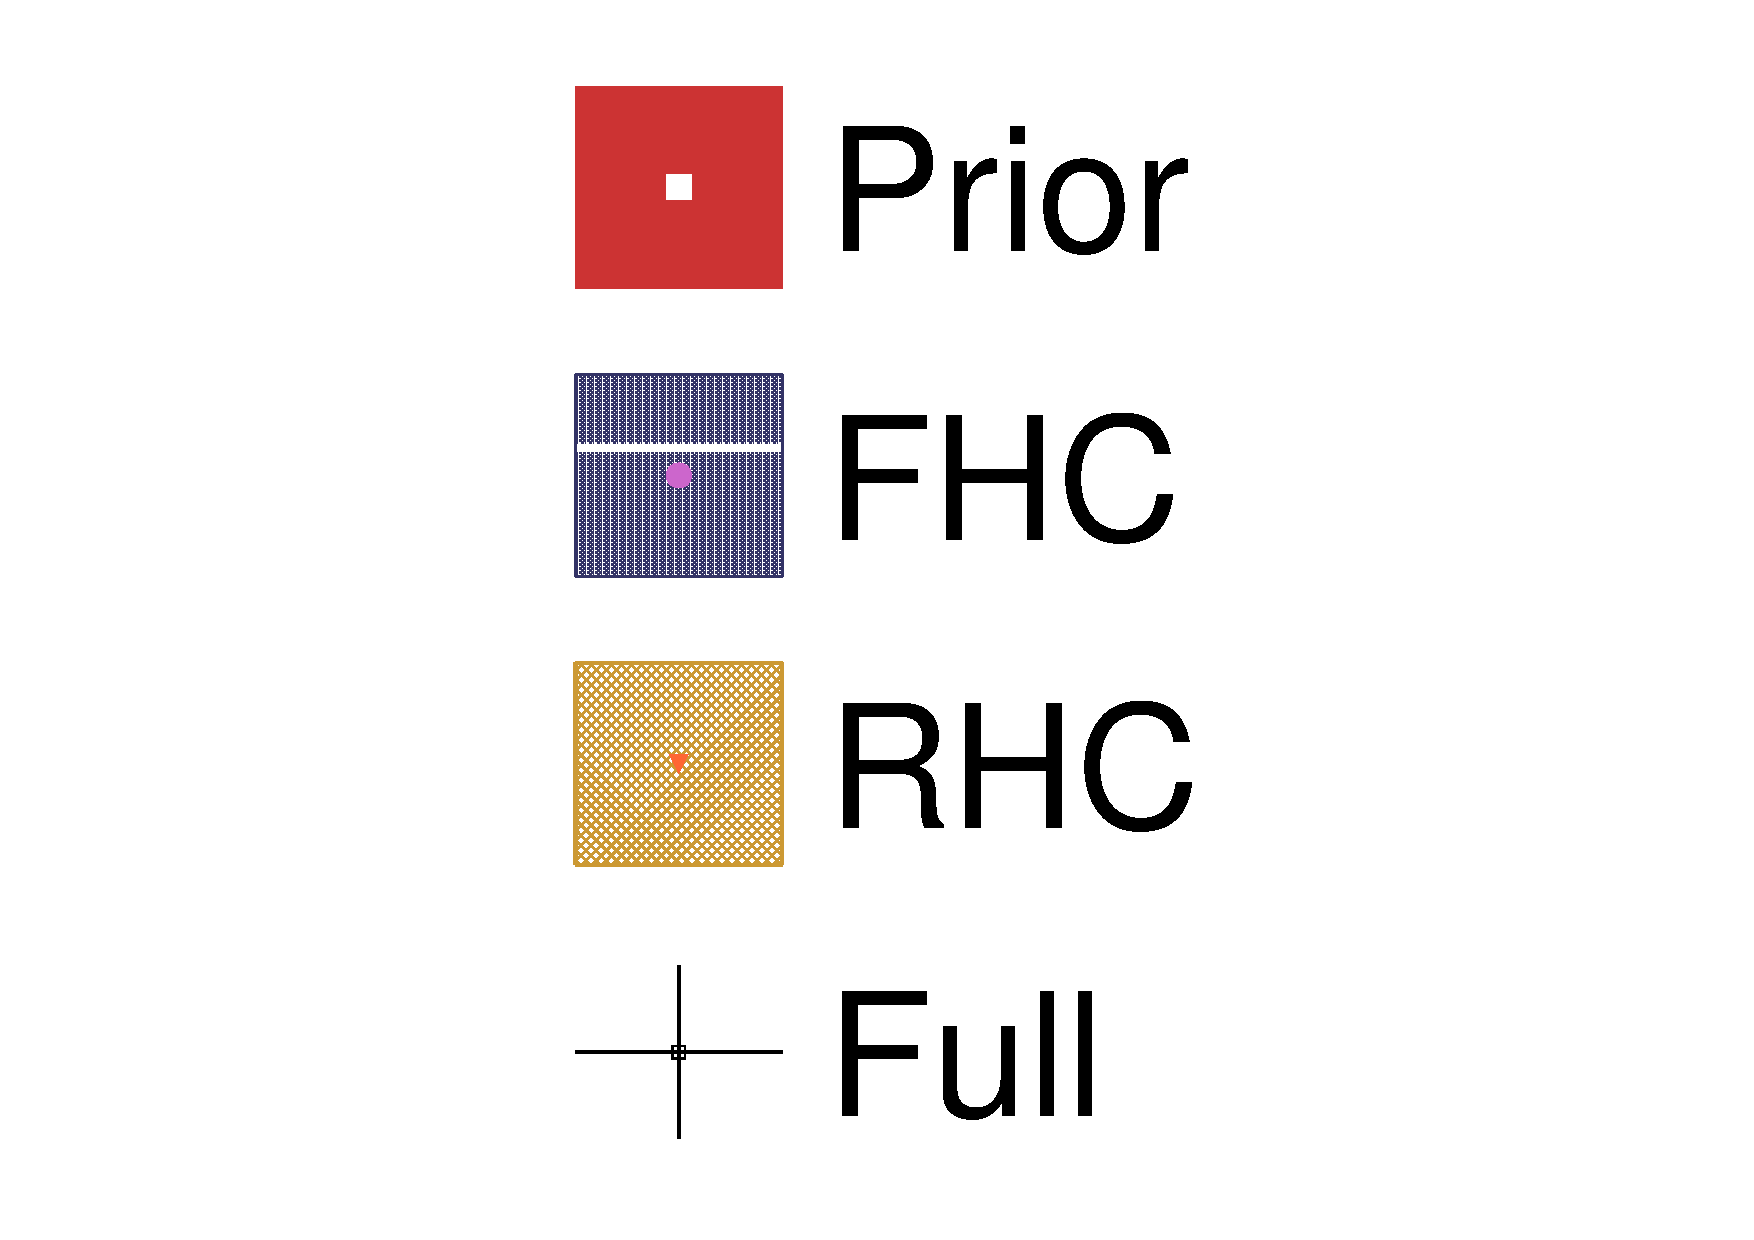
\includegraphics[width=\textwidth,page=1, trim={0mm 0mm 0mm 9mm}, clip]{figures/mach3/2018/data/2018a_FixedCov_RedCov_Mpi_NeuOnly_Data_merge_2018a_FixedCov_RedCov_Mpi_NeuBarOnly_Data_merge_2018a_FixedCov_RedCov_Mpi_Data_merge}
	\end{subfigure}
	
	\begin{subfigure}[t]{\textwidth}
		\begin{subfigure}[t]{0.24\textwidth}
			\includegraphics[width=\textwidth,page=2, trim={0mm 0mm 0mm 9mm}, clip]{figures/mach3/2018/data/2018a_FixedCov_RedCov_Mpi_NeuOnly_Data_merge_2018a_FixedCov_RedCov_Mpi_NeuBarOnly_Data_merge_2018a_FixedCov_RedCov_Mpi_Data_merge}
		\end{subfigure}
		\begin{subfigure}[t]{0.24\textwidth}
			\includegraphics[width=\textwidth,page=3, trim={0mm 0mm 0mm 9mm}, clip]{figures/mach3/2018/data/2018a_FixedCov_RedCov_Mpi_NeuOnly_Data_merge_2018a_FixedCov_RedCov_Mpi_NeuBarOnly_Data_merge_2018a_FixedCov_RedCov_Mpi_Data_merge}
		\end{subfigure}
		\begin{subfigure}[t]{0.24\textwidth}
			\includegraphics[width=\textwidth,page=4, trim={0mm 0mm 0mm 9mm}, clip]{figures/mach3/2018/data/2018a_FixedCov_RedCov_Mpi_NeuOnly_Data_merge_2018a_FixedCov_RedCov_Mpi_NeuBarOnly_Data_merge_2018a_FixedCov_RedCov_Mpi_Data_merge}
		\end{subfigure}
		\begin{subfigure}[t]{0.24\textwidth}
			\includegraphics[width=\textwidth,page=5, trim={0mm 0mm 0mm 9mm}, clip]{figures/mach3/2018/data/2018a_FixedCov_RedCov_Mpi_NeuOnly_Data_merge_2018a_FixedCov_RedCov_Mpi_NeuBarOnly_Data_merge_2018a_FixedCov_RedCov_Mpi_Data_merge}
		\end{subfigure}
		\caption{ND280}
	\end{subfigure}
	
	\begin{subfigure}[t]{\textwidth}
		\begin{subfigure}[t]{0.24\textwidth}
			\includegraphics[width=\textwidth,page=10, trim={0mm 0mm 0mm 9mm}, clip]{figures/mach3/2018/data/2018a_FixedCov_RedCov_Mpi_NeuOnly_Data_merge_2018a_FixedCov_RedCov_Mpi_NeuBarOnly_Data_merge_2018a_FixedCov_RedCov_Mpi_Data_merge}
		\end{subfigure}
		\begin{subfigure}[t]{0.24\textwidth}
			\includegraphics[width=\textwidth,page=11, trim={0mm 0mm 0mm 9mm}, clip]{figures/mach3/2018/data/2018a_FixedCov_RedCov_Mpi_NeuOnly_Data_merge_2018a_FixedCov_RedCov_Mpi_NeuBarOnly_Data_merge_2018a_FixedCov_RedCov_Mpi_Data_merge}
		\end{subfigure}
		\begin{subfigure}[t]{0.24\textwidth}
			\includegraphics[width=\textwidth,page=12, trim={0mm 0mm 0mm 9mm}, clip]{figures/mach3/2018/data/2018a_FixedCov_RedCov_Mpi_NeuOnly_Data_merge_2018a_FixedCov_RedCov_Mpi_NeuBarOnly_Data_merge_2018a_FixedCov_RedCov_Mpi_Data_merge}
		\end{subfigure}
		\begin{subfigure}[t]{0.24\textwidth}
			\includegraphics[width=\textwidth,page=13, trim={0mm 0mm 0mm 9mm}, clip]{figures/mach3/2018/data/2018a_FixedCov_RedCov_Mpi_NeuOnly_Data_merge_2018a_FixedCov_RedCov_Mpi_NeuBarOnly_Data_merge_2018a_FixedCov_RedCov_Mpi_Data_merge}
		\end{subfigure}
		\caption{SK}
	\end{subfigure}
	\caption{FHC flux parameters, fitting to data with different horn configurations}
	\label{fig:data_fhcvsrhc_2018_fhc}
\end{figure}

The RHC parameters in \autoref{fig:data_fhcvsrhc_2018_rhc} show a similar pattern: when the separate FHC and RHC fits prefer a high flux normalisation, the full fit prefers an even higher flux normalisation, and when the two pull away from eachother, the full fit settles in between. The only differences are for the \numubar and \nuebar between 0.4-1.0 GeV, where the RHC fit (which has sample sensitivity to these parameters) sits slightly above the prior and the FHC fit (which only constrains via correlations with the FHC parameters) sits below.
\begin{figure}[h]
	\centering
	\begin{subfigure}[t]{\textwidth}
		\begin{subfigure}[t]{0.24\textwidth}
			\includegraphics[width=\textwidth,page=6, trim={0mm 0mm 0mm 9mm}, clip]{figures/mach3/2018/data/2018a_FixedCov_RedCov_Mpi_NeuOnly_Data_merge_2018a_FixedCov_RedCov_Mpi_NeuBarOnly_Data_merge_2018a_FixedCov_RedCov_Mpi_Data_merge}
		\end{subfigure}
		\begin{subfigure}[t]{0.24\textwidth}
			\includegraphics[width=\textwidth,page=7, trim={0mm 0mm 0mm 9mm}, clip]{figures/mach3/2018/data/2018a_FixedCov_RedCov_Mpi_NeuOnly_Data_merge_2018a_FixedCov_RedCov_Mpi_NeuBarOnly_Data_merge_2018a_FixedCov_RedCov_Mpi_Data_merge}
		\end{subfigure}
		\begin{subfigure}[t]{0.24\textwidth}
			\includegraphics[width=\textwidth,page=8, trim={0mm 0mm 0mm 9mm}, clip]{figures/mach3/2018/data/2018a_FixedCov_RedCov_Mpi_NeuOnly_Data_merge_2018a_FixedCov_RedCov_Mpi_NeuBarOnly_Data_merge_2018a_FixedCov_RedCov_Mpi_Data_merge}
		\end{subfigure}
		\begin{subfigure}[t]{0.24\textwidth}
			\includegraphics[width=\textwidth,page=9, trim={0mm 0mm 0mm 9mm}, clip]{figures/mach3/2018/data/2018a_FixedCov_RedCov_Mpi_NeuOnly_Data_merge_2018a_FixedCov_RedCov_Mpi_NeuBarOnly_Data_merge_2018a_FixedCov_RedCov_Mpi_Data_merge}
		\end{subfigure}
		\caption{ND280}
	\end{subfigure}
	
	\begin{subfigure}[t]{\textwidth}
		\begin{subfigure}[t]{0.24\textwidth}
			\includegraphics[width=\textwidth,page=14, trim={0mm 0mm 0mm 9mm}, clip]{figures/mach3/2018/data/2018a_FixedCov_RedCov_Mpi_NeuOnly_Data_merge_2018a_FixedCov_RedCov_Mpi_NeuBarOnly_Data_merge_2018a_FixedCov_RedCov_Mpi_Data_merge}
		\end{subfigure}
		\begin{subfigure}[t]{0.24\textwidth}
			\includegraphics[width=\textwidth,page=15, trim={0mm 0mm 0mm 9mm}, clip]{figures/mach3/2018/data/2018a_FixedCov_RedCov_Mpi_NeuOnly_Data_merge_2018a_FixedCov_RedCov_Mpi_NeuBarOnly_Data_merge_2018a_FixedCov_RedCov_Mpi_Data_merge}
		\end{subfigure}
		\begin{subfigure}[t]{0.24\textwidth}
			\includegraphics[width=\textwidth,page=16, trim={0mm 0mm 0mm 9mm}, clip]{figures/mach3/2018/data/2018a_FixedCov_RedCov_Mpi_NeuOnly_Data_merge_2018a_FixedCov_RedCov_Mpi_NeuBarOnly_Data_merge_2018a_FixedCov_RedCov_Mpi_Data_merge}
		\end{subfigure}
		\begin{subfigure}[t]{0.24\textwidth}
			\includegraphics[width=\textwidth,page=17, trim={0mm 0mm 0mm 9mm}, clip]{figures/mach3/2018/data/2018a_FixedCov_RedCov_Mpi_NeuOnly_Data_merge_2018a_FixedCov_RedCov_Mpi_NeuBarOnly_Data_merge_2018a_FixedCov_RedCov_Mpi_Data_merge}
		\end{subfigure}
		\caption{SK}
	\end{subfigure}
	\caption{RHC flux parameters, fitting to data with different horn configurations}
	\label{fig:data_fhcvsrhc_2018_rhc}
\end{figure}

The interaction parameters in \autoref{fig:data_fhcvsrhc_2018_xsec} show the largest differences between the two horn configurations. Most CC0$\pi$-related parameters agree up to BeRPA B, which sees a large inflation from the prior, which the RHC data seems to prefer. The full data fit sits right on the FHC-only results, demonstrating the power of the high statistics samples over the prior. The CC0$\pi$ parameters are very similar to the 2017 equivalent results in \autoref{fig:xsec_data_nuvsnubar}.

As in 2017, the single pion parameters are also significantly different for FHC and RHC runs, with the patterns similar but pulls more extreme. Generally the RHC results are closer to the prior. There have already been indications in data\cite{MIN_pion_2016} and modelling\cite{thesis_minoo} that differences in neutrino and anti-neutrino single pion production may be unaccounted for, which here is supported by T2K data.

The remaining differences are found in the pion final state interaction probabilities, where we see weaker constraints from the RHC samples, many times agreeing within 1$\sigma$ with the FHC. As for other parameters where FHC and RHC parameter are in tension, the full fit settles in between with errors to cover the individual fits' 1$\sigma$. The parameters in tension appear to be the inelastic and absorption probabilities, where the RHC selections prefer a higher than nominal value, and FHC the opposite.
\begin{figure}[h]
	\centering
	\begin{subfigure}[t]{0.49\textwidth}
		\includegraphics[width=\textwidth,page=18, trim={0mm 0mm 0mm 9mm}, clip]{figures/mach3/2018/data/2018a_FixedCov_RedCov_Mpi_NeuOnly_Data_merge_2018a_FixedCov_RedCov_Mpi_NeuBarOnly_Data_merge_2018a_FixedCov_RedCov_Mpi_Data_merge}
	\end{subfigure}
	\begin{subfigure}[t]{0.49\textwidth}
		\includegraphics[width=\textwidth,page=19, trim={0mm 0mm 0mm 9mm}, clip]{figures/mach3/2018/data/2018a_FixedCov_RedCov_Mpi_NeuOnly_Data_merge_2018a_FixedCov_RedCov_Mpi_NeuBarOnly_Data_merge_2018a_FixedCov_RedCov_Mpi_Data_merge}
	\end{subfigure}
	
	\begin{subfigure}[t]{0.49\textwidth}
		\includegraphics[width=\textwidth,page=20, trim={0mm 0mm 0mm 9mm}, clip]{figures/mach3/2018/data/2018a_FixedCov_RedCov_Mpi_NeuOnly_Data_merge_2018a_FixedCov_RedCov_Mpi_NeuBarOnly_Data_merge_2018a_FixedCov_RedCov_Mpi_Data_merge}
	\end{subfigure}
	\begin{subfigure}[t]{0.49\textwidth}
		\includegraphics[width=\textwidth,page=21, trim={0mm 0mm 0mm 9mm}, clip]{figures/mach3/2018/data/2018a_FixedCov_RedCov_Mpi_NeuOnly_Data_merge_2018a_FixedCov_RedCov_Mpi_NeuBarOnly_Data_merge_2018a_FixedCov_RedCov_Mpi_Data_merge}
	\end{subfigure}
	\caption{Interaction parameters, fitting to data with different horn configurations}
	\label{fig:data_fhcvsrhc_2018_xsec}
\end{figure}

The different BeRPA parameterisations after fitting FGD1 and FGD2 data are shown in \autoref{fig:data_fhcvsrhc_2018_berpa}. The RHC data clearly prefers a more RPA-like prescription and has larger errors (as expected from the small data set), whereas the FHC data drives the data fit, with an even more extreme enhancement than in 2017 around $Q^2\sim0.5\text{ GeV}^2$.
\begin{figure}[h]
	\centering
	\begin{subfigure}[t]{0.4\textwidth}
		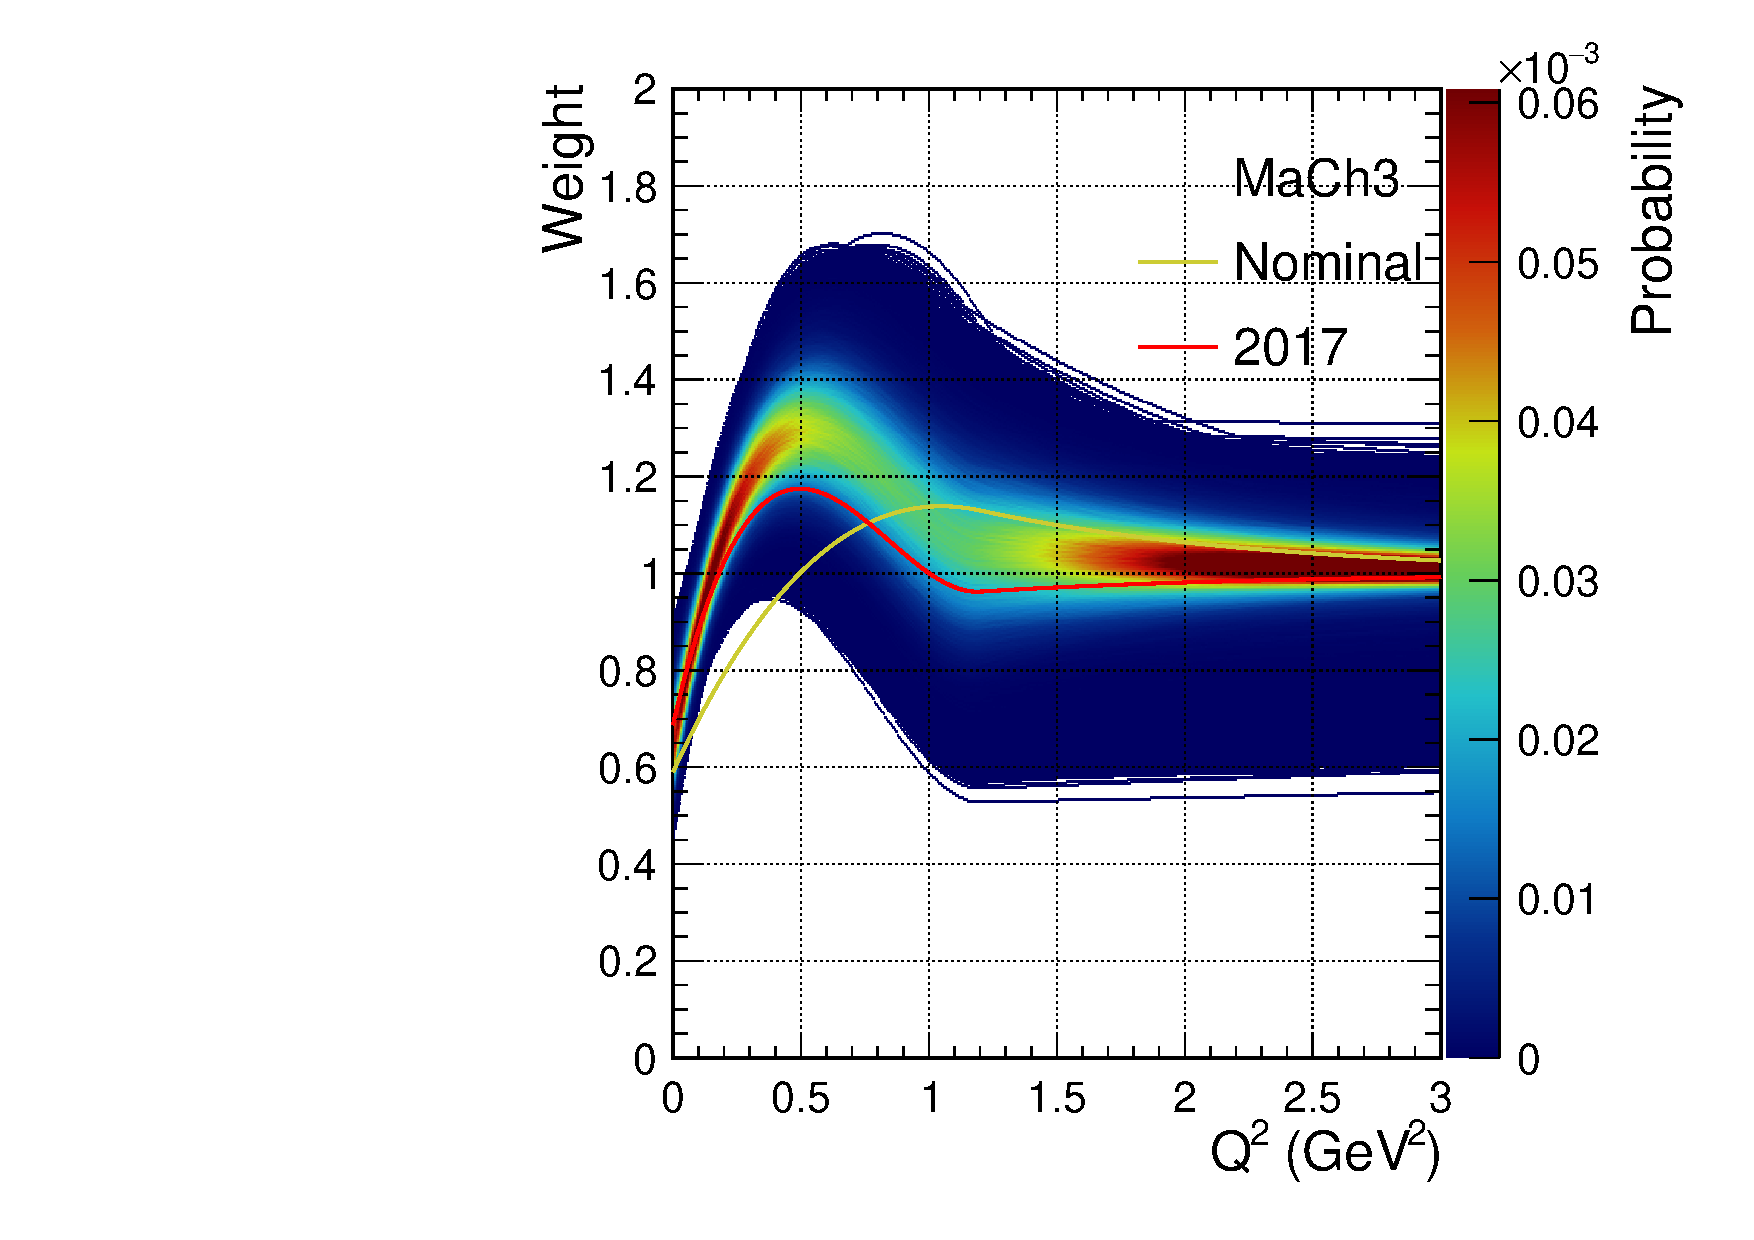
\includegraphics[width=\textwidth,page=1, trim={0mm 0mm 0mm 0mm}, clip]{figures/mach3/2018/data/2018a_MultiPi_Binningv6_NewCov_Data_merge_BeRPA.pdf}
		\caption{FHC}
	\end{subfigure}
	\begin{subfigure}[t]{0.4\textwidth}
		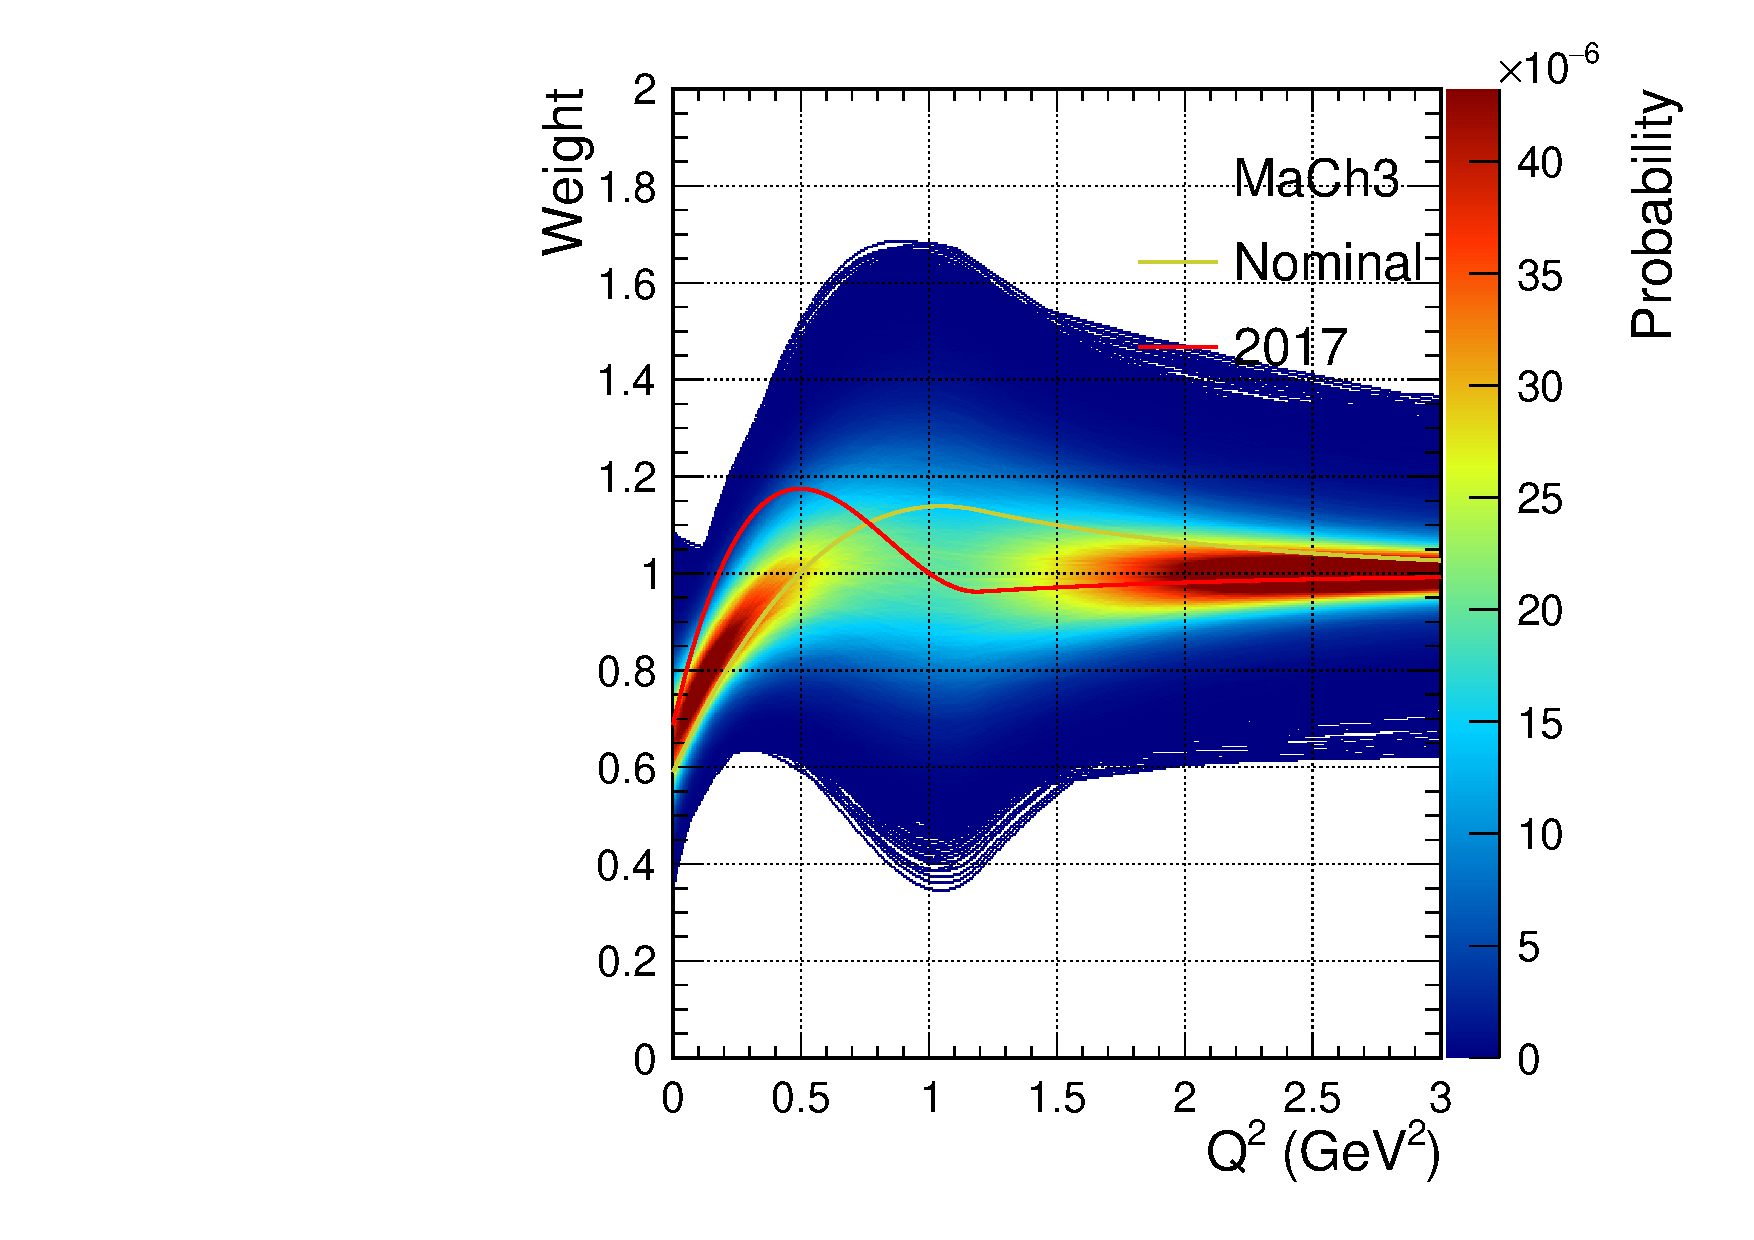
\includegraphics[width=\textwidth,page=1, trim={0mm 0mm 0mm 0mm}, clip]{figures/mach3/2018/data/2018a_FixedCov_RedCov_Mpi_NeuBarOnly_Data_merge_BeRPA.pdf}
		\caption{RHC}
	\end{subfigure}
	\caption{BeRPA parameterisations for fitting to data with different horn configurations}
	\label{fig:data_fhcvsrhc_2018_berpa}
\end{figure}

As with the 2017 analysis, comparing neutrino and anti-neutrino fits to the full fit has highlighted differences in BeRPA, single pion production and pion FSI probabilities. The tensions from 2017 seem to remain in the larger 2018 fit and should be addressed in the future.

\section{FGD1 vs FGD2}
We now compare using FGD1 and FGD2 selections to using both, identical to in 2017. The 2017 analysis saw relatively large differences in the flux parameters, notably at high $E_\nu$, and the interaction parameters had different $M_A^{QE}$ and BeRPA B values.

The FHC flux parameter are shown in \autoref{fig:data_fdg1vsfgd2_2018_fhc} where we mostly see compatibility. Similar to the FHC vs RHC case, the full FGD1+FGD2 fit favours a higher flux at low $E_\nu$ than the separate FGD1 and FGD2 fits, which is repeated whenever the flux parameter values are high. The results are generally compatible.
\begin{figure}[h]
	\centering
	\begin{subfigure}[t]{0.10\textwidth}
		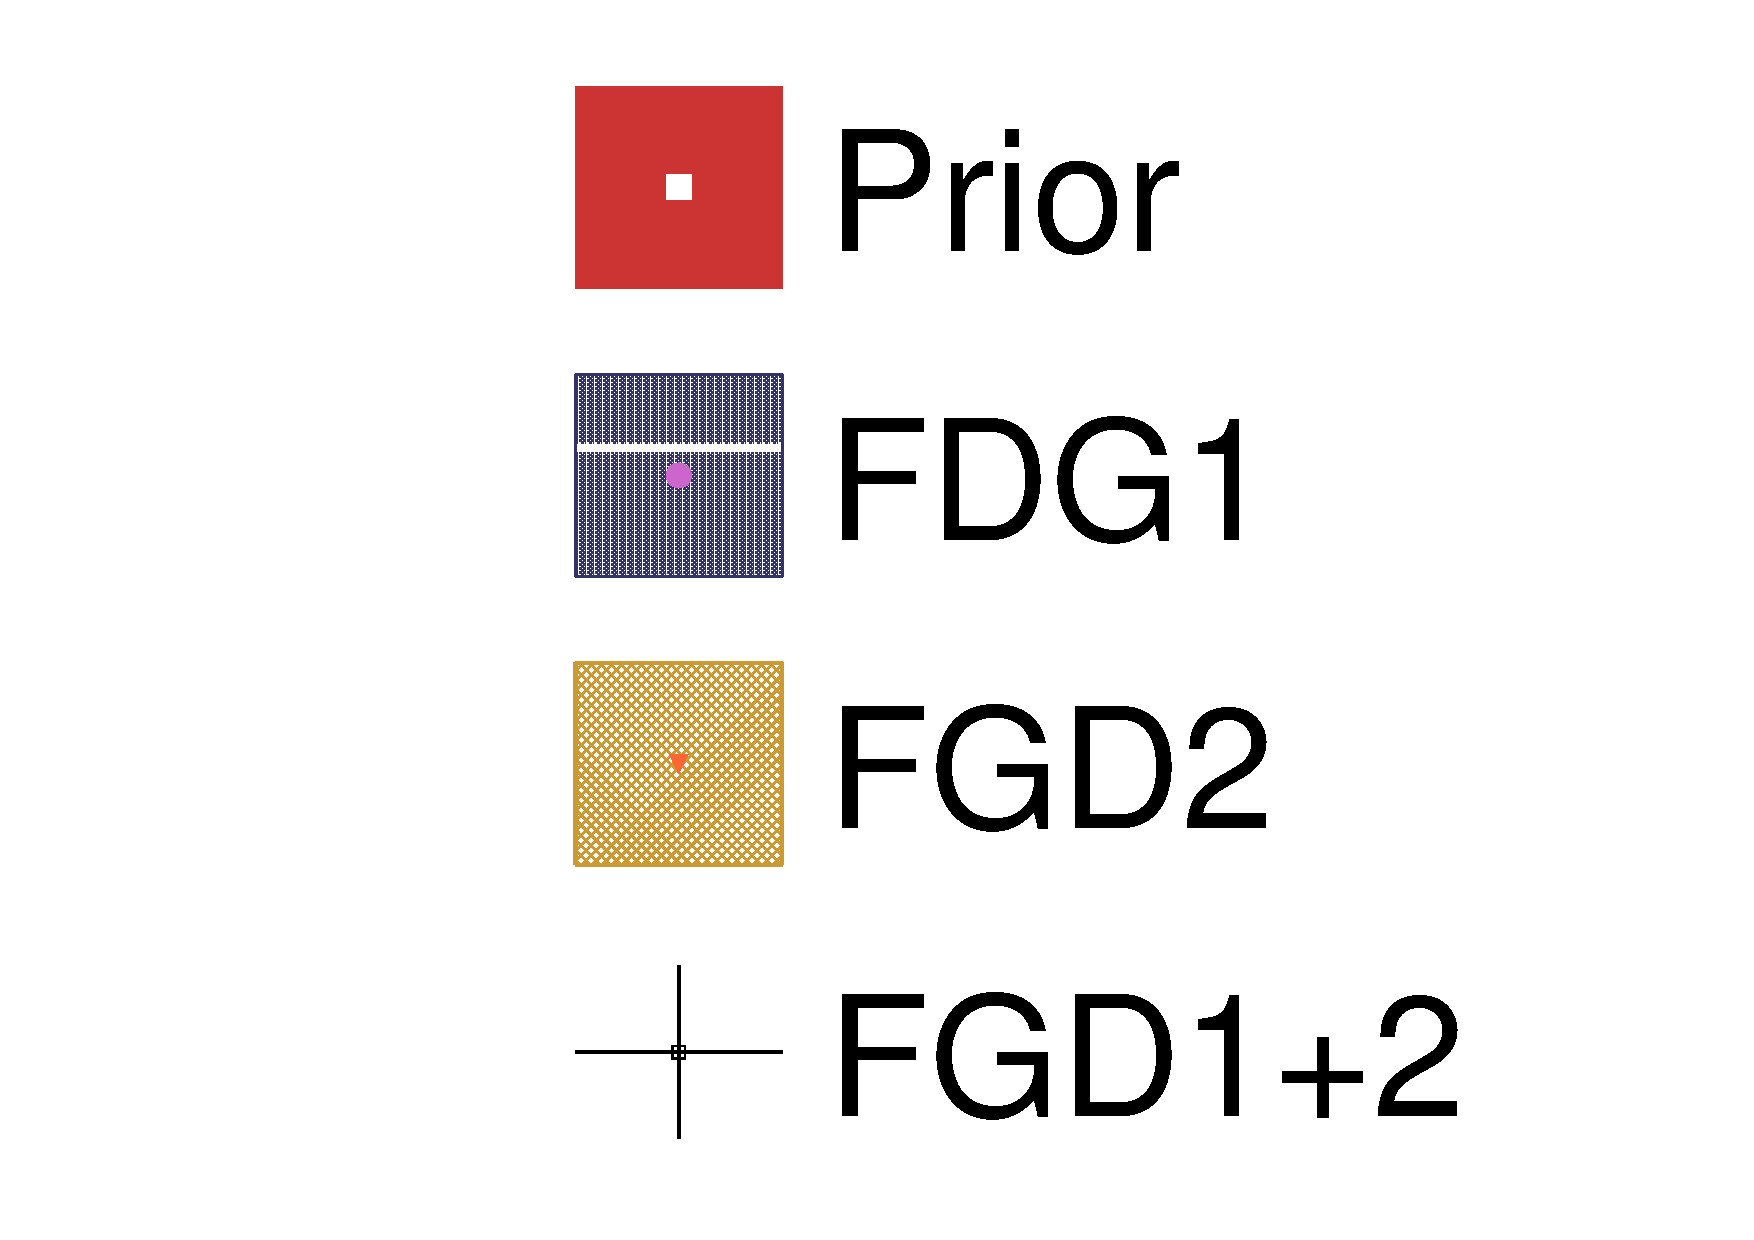
\includegraphics[width=\textwidth,page=1, trim={0mm 0mm 0mm 9mm}, clip]{figures/mach3/2018/data/2018a_FixedCov_RedCov_Mpi_FGD1Only_Data_merge_2018a_FixedCov_RedCov_Mpi_FGD2Only_Data_merge_2018a_FixedCov_RedCov_Mpi_Data_merge}
	\end{subfigure}
	
	\begin{subfigure}[t]{\textwidth}
		\begin{subfigure}[t]{0.24\textwidth}
			\includegraphics[width=\textwidth,page=2, trim={0mm 0mm 0mm 9mm}, clip]{figures/mach3/2018/data/2018a_FixedCov_RedCov_Mpi_FGD1Only_Data_merge_2018a_FixedCov_RedCov_Mpi_FGD2Only_Data_merge_2018a_FixedCov_RedCov_Mpi_Data_merge}
		\end{subfigure}
		\begin{subfigure}[t]{0.24\textwidth}
			\includegraphics[width=\textwidth,page=3, trim={0mm 0mm 0mm 9mm}, clip]{figures/mach3/2018/data/2018a_FixedCov_RedCov_Mpi_FGD1Only_Data_merge_2018a_FixedCov_RedCov_Mpi_FGD2Only_Data_merge_2018a_FixedCov_RedCov_Mpi_Data_merge}
		\end{subfigure}
		\begin{subfigure}[t]{0.24\textwidth}
			\includegraphics[width=\textwidth,page=4, trim={0mm 0mm 0mm 9mm}, clip]{figures/mach3/2018/data/2018a_FixedCov_RedCov_Mpi_FGD1Only_Data_merge_2018a_FixedCov_RedCov_Mpi_FGD2Only_Data_merge_2018a_FixedCov_RedCov_Mpi_Data_merge}
		\end{subfigure}
		\begin{subfigure}[t]{0.24\textwidth}
			\includegraphics[width=\textwidth,page=5, trim={0mm 0mm 0mm 9mm}, clip]{figures/mach3/2018/data/2018a_FixedCov_RedCov_Mpi_FGD1Only_Data_merge_2018a_FixedCov_RedCov_Mpi_FGD2Only_Data_merge_2018a_FixedCov_RedCov_Mpi_Data_merge}
		\end{subfigure}
		\caption{ND280}
	\end{subfigure}
	
	\begin{subfigure}[t]{\textwidth}
		\begin{subfigure}[t]{0.24\textwidth}
			\includegraphics[width=\textwidth,page=10, trim={0mm 0mm 0mm 9mm}, clip]{figures/mach3/2018/data/2018a_FixedCov_RedCov_Mpi_FGD1Only_Data_merge_2018a_FixedCov_RedCov_Mpi_FGD2Only_Data_merge_2018a_FixedCov_RedCov_Mpi_Data_merge}
		\end{subfigure}
		\begin{subfigure}[t]{0.24\textwidth}
			\includegraphics[width=\textwidth,page=11, trim={0mm 0mm 0mm 9mm}, clip]{figures/mach3/2018/data/2018a_FixedCov_RedCov_Mpi_FGD1Only_Data_merge_2018a_FixedCov_RedCov_Mpi_FGD2Only_Data_merge_2018a_FixedCov_RedCov_Mpi_Data_merge}
		\end{subfigure}
		\begin{subfigure}[t]{0.24\textwidth}
			\includegraphics[width=\textwidth,page=12, trim={0mm 0mm 0mm 9mm}, clip]{figures/mach3/2018/data/2018a_FixedCov_RedCov_Mpi_FGD1Only_Data_merge_2018a_FixedCov_RedCov_Mpi_FGD2Only_Data_merge_2018a_FixedCov_RedCov_Mpi_Data_merge}
		\end{subfigure}
		\begin{subfigure}[t]{0.24\textwidth}
			\includegraphics[width=\textwidth,page=13, trim={0mm 0mm 0mm 9mm}, clip]{figures/mach3/2018/data/2018a_FixedCov_RedCov_Mpi_FGD1Only_Data_merge_2018a_FixedCov_RedCov_Mpi_FGD2Only_Data_merge_2018a_FixedCov_RedCov_Mpi_Data_merge}
		\end{subfigure}
		\caption{SK}
	\end{subfigure}
	
	\caption{FHC flux parameters, fitting to data with FGD1 and FGD2}
	\label{fig:data_fdg1vsfgd2_2018_fhc}
\end{figure}

For the RHC flux parameters in \autoref{fig:data_fdg1vsfgd2_2018_fhc} the compatibility is also good with the same patterns repeated.
\begin{figure}[h]
	\centering
	\begin{subfigure}[t]{\textwidth}
		\begin{subfigure}[t]{0.24\textwidth}
			\includegraphics[width=\textwidth,page=6, trim={0mm 0mm 0mm 9mm}, clip]{figures/mach3/2018/data/2018a_FixedCov_RedCov_Mpi_FGD1Only_Data_merge_2018a_FixedCov_RedCov_Mpi_FGD2Only_Data_merge_2018a_FixedCov_RedCov_Mpi_Data_merge}
		\end{subfigure}
		\begin{subfigure}[t]{0.24\textwidth}
			\includegraphics[width=\textwidth,page=7, trim={0mm 0mm 0mm 9mm}, clip]{figures/mach3/2018/data/2018a_FixedCov_RedCov_Mpi_FGD1Only_Data_merge_2018a_FixedCov_RedCov_Mpi_FGD2Only_Data_merge_2018a_FixedCov_RedCov_Mpi_Data_merge}
		\end{subfigure}
		\begin{subfigure}[t]{0.24\textwidth}
			\includegraphics[width=\textwidth,page=8, trim={0mm 0mm 0mm 9mm}, clip]{figures/mach3/2018/data/2018a_FixedCov_RedCov_Mpi_FGD1Only_Data_merge_2018a_FixedCov_RedCov_Mpi_FGD2Only_Data_merge_2018a_FixedCov_RedCov_Mpi_Data_merge}
		\end{subfigure}
		\begin{subfigure}[t]{0.24\textwidth}
			\includegraphics[width=\textwidth,page=9, trim={0mm 0mm 0mm 9mm}, clip]{figures/mach3/2018/data/2018a_FixedCov_RedCov_Mpi_FGD1Only_Data_merge_2018a_FixedCov_RedCov_Mpi_FGD2Only_Data_merge_2018a_FixedCov_RedCov_Mpi_Data_merge}
		\end{subfigure}
		\caption{ND280}
	\end{subfigure}
	
	\begin{subfigure}[t]{\textwidth}
		\begin{subfigure}[t]{0.24\textwidth}
			\includegraphics[width=\textwidth,page=14, trim={0mm 0mm 0mm 9mm}, clip]{figures/mach3/2018/data/2018a_FixedCov_RedCov_Mpi_FGD1Only_Data_merge_2018a_FixedCov_RedCov_Mpi_FGD2Only_Data_merge_2018a_FixedCov_RedCov_Mpi_Data_merge}
		\end{subfigure}
		\begin{subfigure}[t]{0.24\textwidth}
			\includegraphics[width=\textwidth,page=15, trim={0mm 0mm 0mm 9mm}, clip]{figures/mach3/2018/data/2018a_FixedCov_RedCov_Mpi_FGD1Only_Data_merge_2018a_FixedCov_RedCov_Mpi_FGD2Only_Data_merge_2018a_FixedCov_RedCov_Mpi_Data_merge}
		\end{subfigure}
		\begin{subfigure}[t]{0.24\textwidth}
			\includegraphics[width=\textwidth,page=16, trim={0mm 0mm 0mm 9mm}, clip]{figures/mach3/2018/data/2018a_FixedCov_RedCov_Mpi_FGD1Only_Data_merge_2018a_FixedCov_RedCov_Mpi_FGD2Only_Data_merge_2018a_FixedCov_RedCov_Mpi_Data_merge}
		\end{subfigure}
		\begin{subfigure}[t]{0.24\textwidth}
			\includegraphics[width=\textwidth,page=17, trim={0mm 0mm 0mm 9mm}, clip]{figures/mach3/2018/data/2018a_FixedCov_RedCov_Mpi_FGD1Only_Data_merge_2018a_FixedCov_RedCov_Mpi_FGD2Only_Data_merge_2018a_FixedCov_RedCov_Mpi_Data_merge}
		\end{subfigure}
		\caption{SK}
	\end{subfigure}
	\caption{RHC flux parameters, fitting to data with FGD1 and FGD2}
	\label{fig:data_fdg1vsfgd2_2018_rhc}
\end{figure}

The interaction parameters in \autoref{fig:data_fdg1vsfgd2_2018_xsec} are also more compatible than in 2017, but show some similarities. Notably $M_A^{QE}$ is again different for FGD1 and FGD2, with FGD1 favouring an inflated ``MiniBooNE-like'' value ($\sim1.2\text{ GeV}$) and FGD2 a more bubble-chamber like value ($\sim1.0\text{ GeV}$). The 2p2h shape C parameter is slightly different (although within error) and the full fit settles closer to the FGD2 fitted value than FGD1. The BeRPA parameters are compatible, with the largerst difference in BeRPA D, which controls the behaviour around 0.8-1.0 $\text{GeV}^2$. 

There is some tension in the $C_5^A$ single pion production parameter, where FGD1 favours a value agreeing with the prior and FGD2 below that. This was seen in 2017 also, and was correlated with the differences in single pion production parameters. Both FGDs prefer a non-resonant $I_{1/2}$ background higher than nominal, with FGD2 inflating it by 200\% (or 140\% of nominal), again indicating insufficient single pion modelling.

The pion final state parameters are also mostly compatible with the 2017 fit, where FGD1 often prefers a larger parameter value than FGD2. The pion charge exchange parameter is the first time the new FSI parameter priors are pulled outside the 1$\sigma$, although FGD2 prefers a value much in-line with the prior.
\begin{figure}[h]
	\centering
	\begin{subfigure}[t]{0.49\textwidth}
		\includegraphics[width=\textwidth,page=18, trim={0mm 0mm 0mm 9mm}, clip]{figures/mach3/2018/data/2018a_FixedCov_RedCov_Mpi_FGD1Only_Data_merge_2018a_FixedCov_RedCov_Mpi_FGD2Only_Data_merge_2018a_FixedCov_RedCov_Mpi_Data_merge}
	\end{subfigure}
	\begin{subfigure}[t]{0.49\textwidth}
		\includegraphics[width=\textwidth,page=19, trim={0mm 0mm 0mm 9mm}, clip]{figures/mach3/2018/data/2018a_FixedCov_RedCov_Mpi_FGD1Only_Data_merge_2018a_FixedCov_RedCov_Mpi_FGD2Only_Data_merge_2018a_FixedCov_RedCov_Mpi_Data_merge}
	\end{subfigure}
	
	\begin{subfigure}[t]{0.49\textwidth}
		\includegraphics[width=\textwidth,page=20, trim={0mm 0mm 0mm 9mm}, clip]{figures/mach3/2018/data/2018a_FixedCov_RedCov_Mpi_FGD1Only_Data_merge_2018a_FixedCov_RedCov_Mpi_FGD2Only_Data_merge_2018a_FixedCov_RedCov_Mpi_Data_merge}
	\end{subfigure}
	\begin{subfigure}[t]{0.49\textwidth}
		\includegraphics[width=\textwidth,page=21, trim={0mm 0mm 0mm 9mm}, clip]{figures/mach3/2018/data/2018a_FixedCov_RedCov_Mpi_FGD1Only_Data_merge_2018a_FixedCov_RedCov_Mpi_FGD2Only_Data_merge_2018a_FixedCov_RedCov_Mpi_Data_merge}
	\end{subfigure}
	\caption{Interaction parameters, fitting to data with FGD1 and FGD2}
	\label{fig:data_fdg1vsfgd2_2018_xsec}
\end{figure}

In conclusion, the FGD1 vs FGD2 compatibility largely agrees with the 2017 conclusions, with better agreement in the flux parameters. $M_A^{QE}$ and BeRPA D are the largest CC0$\pi$ differences, and the single pion parameters and pion FSI are pulled differently too. Throughout, all the parameters are within 1$\sigma$ of the full fit (and often of each other).

